\section{Uniform approximation}


\begin{exercise}{1}
If $Y \subseteq C[a,b]$ is a subspace of dimension $n$ and satisfies the Haar condition, show that the restrictions of the elements of $Y$ to any subset of $[a,b]$ consisting of $n$ points constitute a vector space which still has dimension $n$ (whereas ordinarily the dimension would decrease under such a restriction).
\end{exercise}
\begin{proof}
This is a Corollary to the determinant version of the Haar condition, which state that for every $n$-tuple of distinct points $t_1, \dots t_n$ in $[a,b]$, the matrix with $i$-th row $(y_i(t_1), \dots, y_i(t_n))$, for a basis $(y_1, \dots, y_n)$ of $Y$ has determinant zero.
Thus, the corresponding matrix of the basis of $Y$ restricted to those points will still have non zero determinant, so that the columns of the matrix are linearly independent and thus the space will still have dimension $n$.
\end{proof} 

\begin{exercise}{2}
Let $x_1(t) = 1$ and $x_2(t) = t^2$.
Does $Y = \vecspan \set{x_1, x_2}$ satisfy the Haar condition if $Y$ is regarded as a subspace 
\begin{enumerate}
    \item of $C[0,1]$,
    \item of $C[-1, 1]$?
\end{enumerate}
(To understand what is going on, approximate $x$ defined by $x(t) = t^3$ in both cases).
\end{exercise}
\begin{proof}
\begin{enumerate}
    \item It does, because for any $y \in Y$ we write $y = a_1 + a_2 t^2$, which has only one root in $[0,1]$, for all values of $a_1$ and $a_2$.
    \item It doesn't.
    Consider $y = -1 + t^2$, which has two roots:
    $-1$ and $1$.
\end{enumerate}
\end{proof} 

\begin{exercise}{3}
Show that $Y \vecspan \set{y_1, \dots, y_n} \subseteq C[a,b]$ satisfies the Haar condition if and only if, for every $n$-tuple $\set{t_1, \dots, t_n} \subset C[a,b]$ consisting of $n$ different points, the $n$ vectors $v_j = (y_1(t_j), \dots, y_n(t_j))$, $j = 1, \dots, n$, form a linearly independent set.
\end{exercise}
\begin{proof}
This is precisely the condition after definition 6.3.2, that is, the matrix $n$ by $n$ matrix with rows $y_i(t_1), y_i(t_2) \dots, y_i(t_n)$ has determinant zero if and only if its columns are linearly independent, which is the same as $v_1, \dots, v_n$ being linearly independent.
\end{proof} 

\begin{exercise}{6}
In $C[0,1]$ find the best approximation to $f$ defined by $f(x) = e^x$ out of $Y = \vecspan \set{y_1, y_2}$, where $g_1(x) = 1$, $g_2(x) = x$.
Compare the approximation with that by the linear Taylor polynomial given by $1+x$.
\end{exercise}
\begin{proof}
For this exercise, I will not find the best approximation by hand, instead I will use the Remez algorithm which I coded in Python and I describe below.
Suppose we want to approximate $f(x)$ in $C[a,b]$ with a polynomial of degree $n$.

\begin{enumerate}
    \item Initialize $n+2$ points using the Chebyshev nodes:
    \begin{align*}
        x_i = \cos\parens{\frac{K - 1 - i}{K - 1}},
    \end{align*}
    for $i = 0, 1, \dots n+1$ and $K = n+2$.
    These nodes are initialized in the $[-1, 1]$ interval so we transform them into $[a,b]$ with 
    \begin{align*}
        x_i := a + \frac{b-a}{2}(x_i + 1).
    \end{align*}
    \item Using these nodes, find the solution to the system of linear equations given by 
    $a_0 + a_1 x_i + a_2 x_i^2 + \dots + (-1)^i E = f(x_i)$, for $i = 0, 1, \dots, n+1$.
    This will give us $a_0, \dots, a_n, E$.
    \item We build the error function $E(x) = f(x) - P(x)$, where $P(x)$ is the polynomial using the coefficients we found in the previous step.
    \item Find the extremum of $\absoluteValue{E(x)}$, say $x'$, and replace with the closest node with the same sign as $E(x')$. 
    \item With the new set of nodes, repeat the process until some convergence criterion is reached.
\end{enumerate}
The found approximation is depicted in \Cref{fig:sec6-3-ex6}.
\begin{figure}
    \centering
    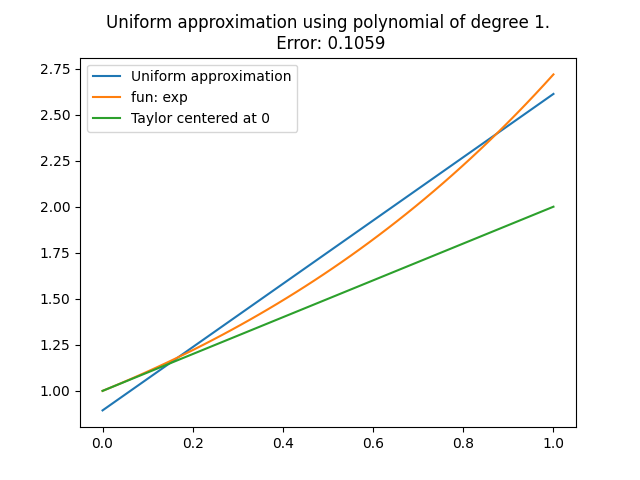
\includegraphics[width=\linewidth]{kreyszig/assets/sec6-3-ex6.png}
    \caption{Uniform approximation of $e^x$ on $[0,1]$ using a polynomial of degree 1.}
    \label{fig:sec6-3-ex6}
\end{figure}
\end{proof} 

\begin{exercise}{9 (Inconsistent linear equation)}
If a system of $r > n$ linear equations in $n$ unknowns $a_{j 1} x_1 + a_{j 2} x_2 + \dots + a_{j n} x_n = b_j$ ($j = 1, \dots, r$) is inconsistent, it does not have a solution $x = (x_1, \dots, x_n)$ but we can look for an `approximate solution' $y = (y_1, \dots, y_n)$ such that $\max \absoluteValue{b_j - \sum_k a_{j k} y_k}$ is as small as possible.
How does this problem fit into our present consideration and what form does the Haar condition take in this case?
\end{exercise}
\begin{proof}
We are looking for an element $(y_1, \dots, y_n)$ of a subspace $Y$ (of dimension $n$) which approximates $b$ uniformly (where the dimension where $b$ lies is $r > n$).
As such this is an approximation problem.

For the Haar condition, we can think in a similar was as in exercise 1.
We take any $n \times n$ submatrix of the matrix defined by the $a_{i,j}$ coefficients, and that submatrix should have linearly independent columns.
\end{proof} 
